\documentclass[a4paper]{article}
\usepackage[T1]{fontenc}
\usepackage[russian]{babel}
\usepackage[pdftex]{graphicx}
\usepackage[ruled,vlined]{algorithm2e}
\usepackage[utf8]{inputenc}
\usepackage{xcolor}
\usepackage{hyperref}
\usepackage{amsmath}
\usepackage{geometry}
\usepackage{float}
\usepackage{caption}
\usepackage{subcaption}
\DeclareGraphicsExtensions{.pdf,.png,.jpg}

\begin{document}

    \begin{titlepage}
        \Large
        \begin{center}
            Санкт-Петербургский \ Политехнический университет Петра Великого\\
            \vspace{10em}Отчет по лабораторной работе №2\\
            \vspace{2em}
            \textbf{Анализ выбросов в распределениях}
        \end{center}
        \vspace{6em}
        \hfill\parbox{10cm}{
            \hspace*{2cm}\hspace*{-4cm}Студент:\hfill Швачко Никита Андреевич\\
            \hspace*{2cm}\hspace*{-4cm}Преподаватель:\hfill Баженов Александр Николаевич\\
            \hspace*{2cm}\hspace*{-4cm}Группа:\hfill 5030102/20202
        }
        \vspace{\fill}
        \begin{center}
            Санкт-Петербург \ 2025
        \end{center}
    \end{titlepage}


    \section{Формулировка задания и его формализация}\label{sec:task}
    Для 4 распределений:
    \begin{itemize}
        \item Нормальное распределение $N(x, 0,1)$
        \item Распределение Коши $C(x, 0,1)$
        \item Распределение Пуассона $P(k, 10)$
        \item Равномерное распределение $U(x,-\sqrt{3}, \sqrt{3})$
    \end{itemize}
    Необходимо:
    \begin{enumerate}
        \item Сгенерировать выборки размером 20, 100 и 1000 элементов.
        \item Построить для каждой выборки боксплоты Тьюки.
        \item Определить количество выбросов в каждой выборке.
        \item Представить данные в таблице и сделать выводы.
    \end{enumerate}


    \section{Boxplot-диаграммы распределений}\label{sec:boxplots}
    \begin{figure}[H]
        \centering
        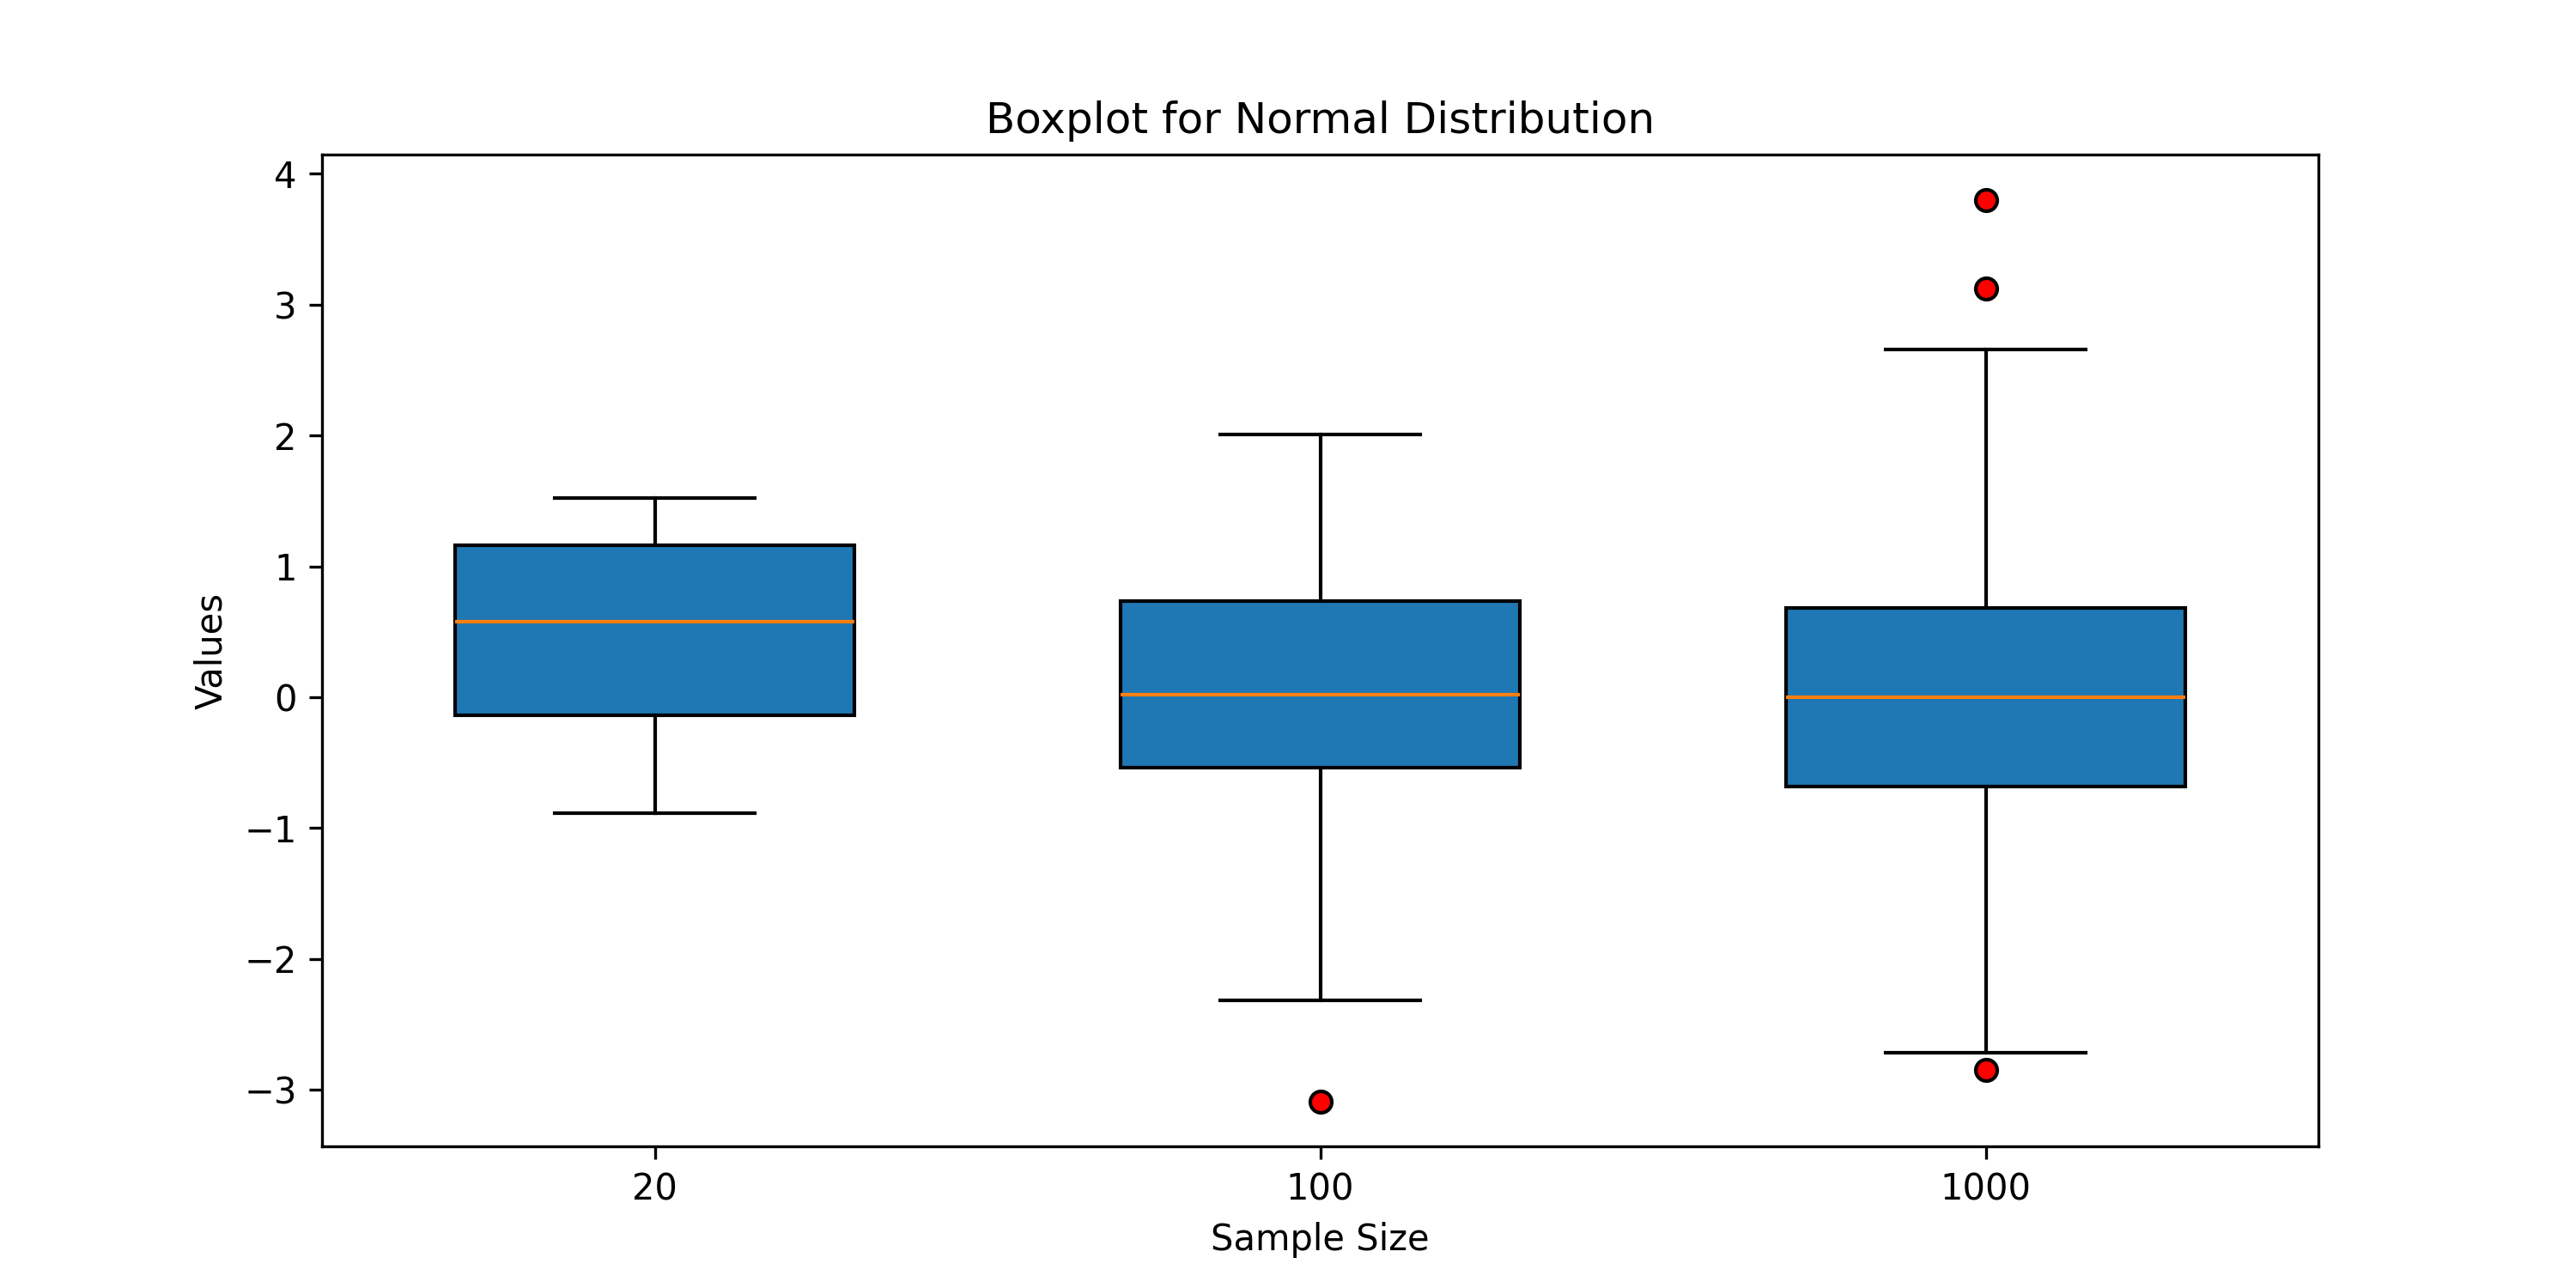
\includegraphics[width=0.8\textwidth]{./plots/normal_boxplot}
        \caption{Боксплот Тьюки для нормального распределения}
        \label{fig:normal_boxplot}
    \end{figure}

    \begin{figure}[H]
        \centering
        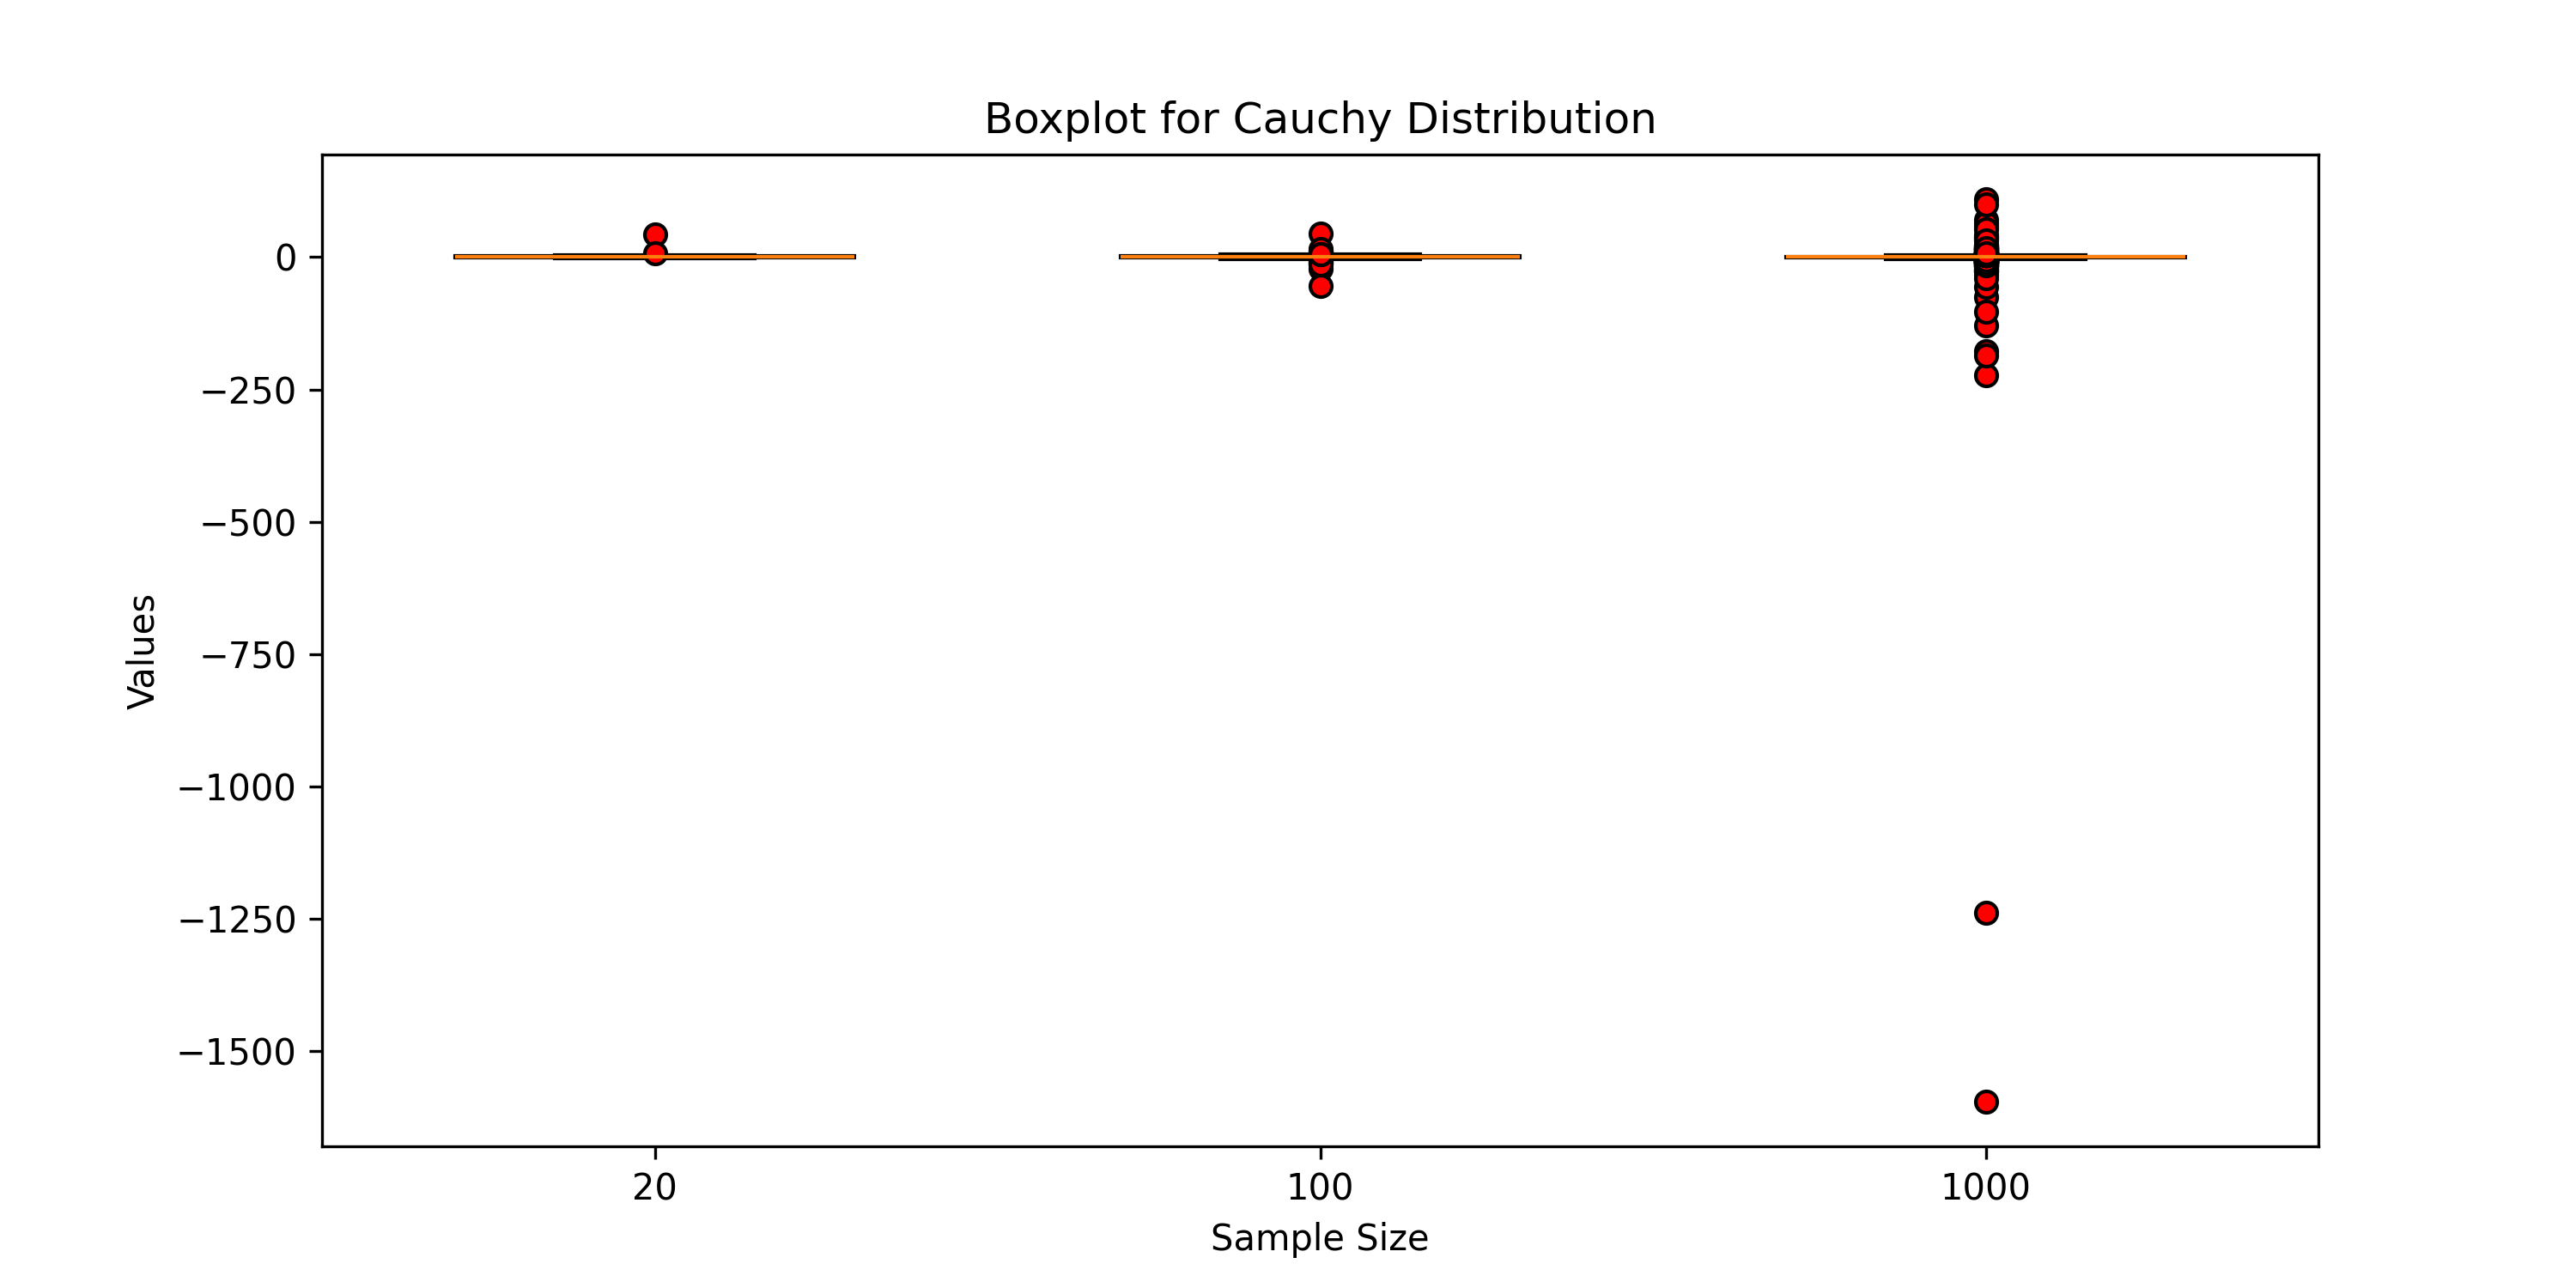
\includegraphics[width=0.8\textwidth]{./plots/cauchy_boxplot}
        \caption{Боксплот Тьюки для распределения Коши}
        \label{fig:cauchy_boxplot}
    \end{figure}

    \begin{figure}[H]
        \centering
        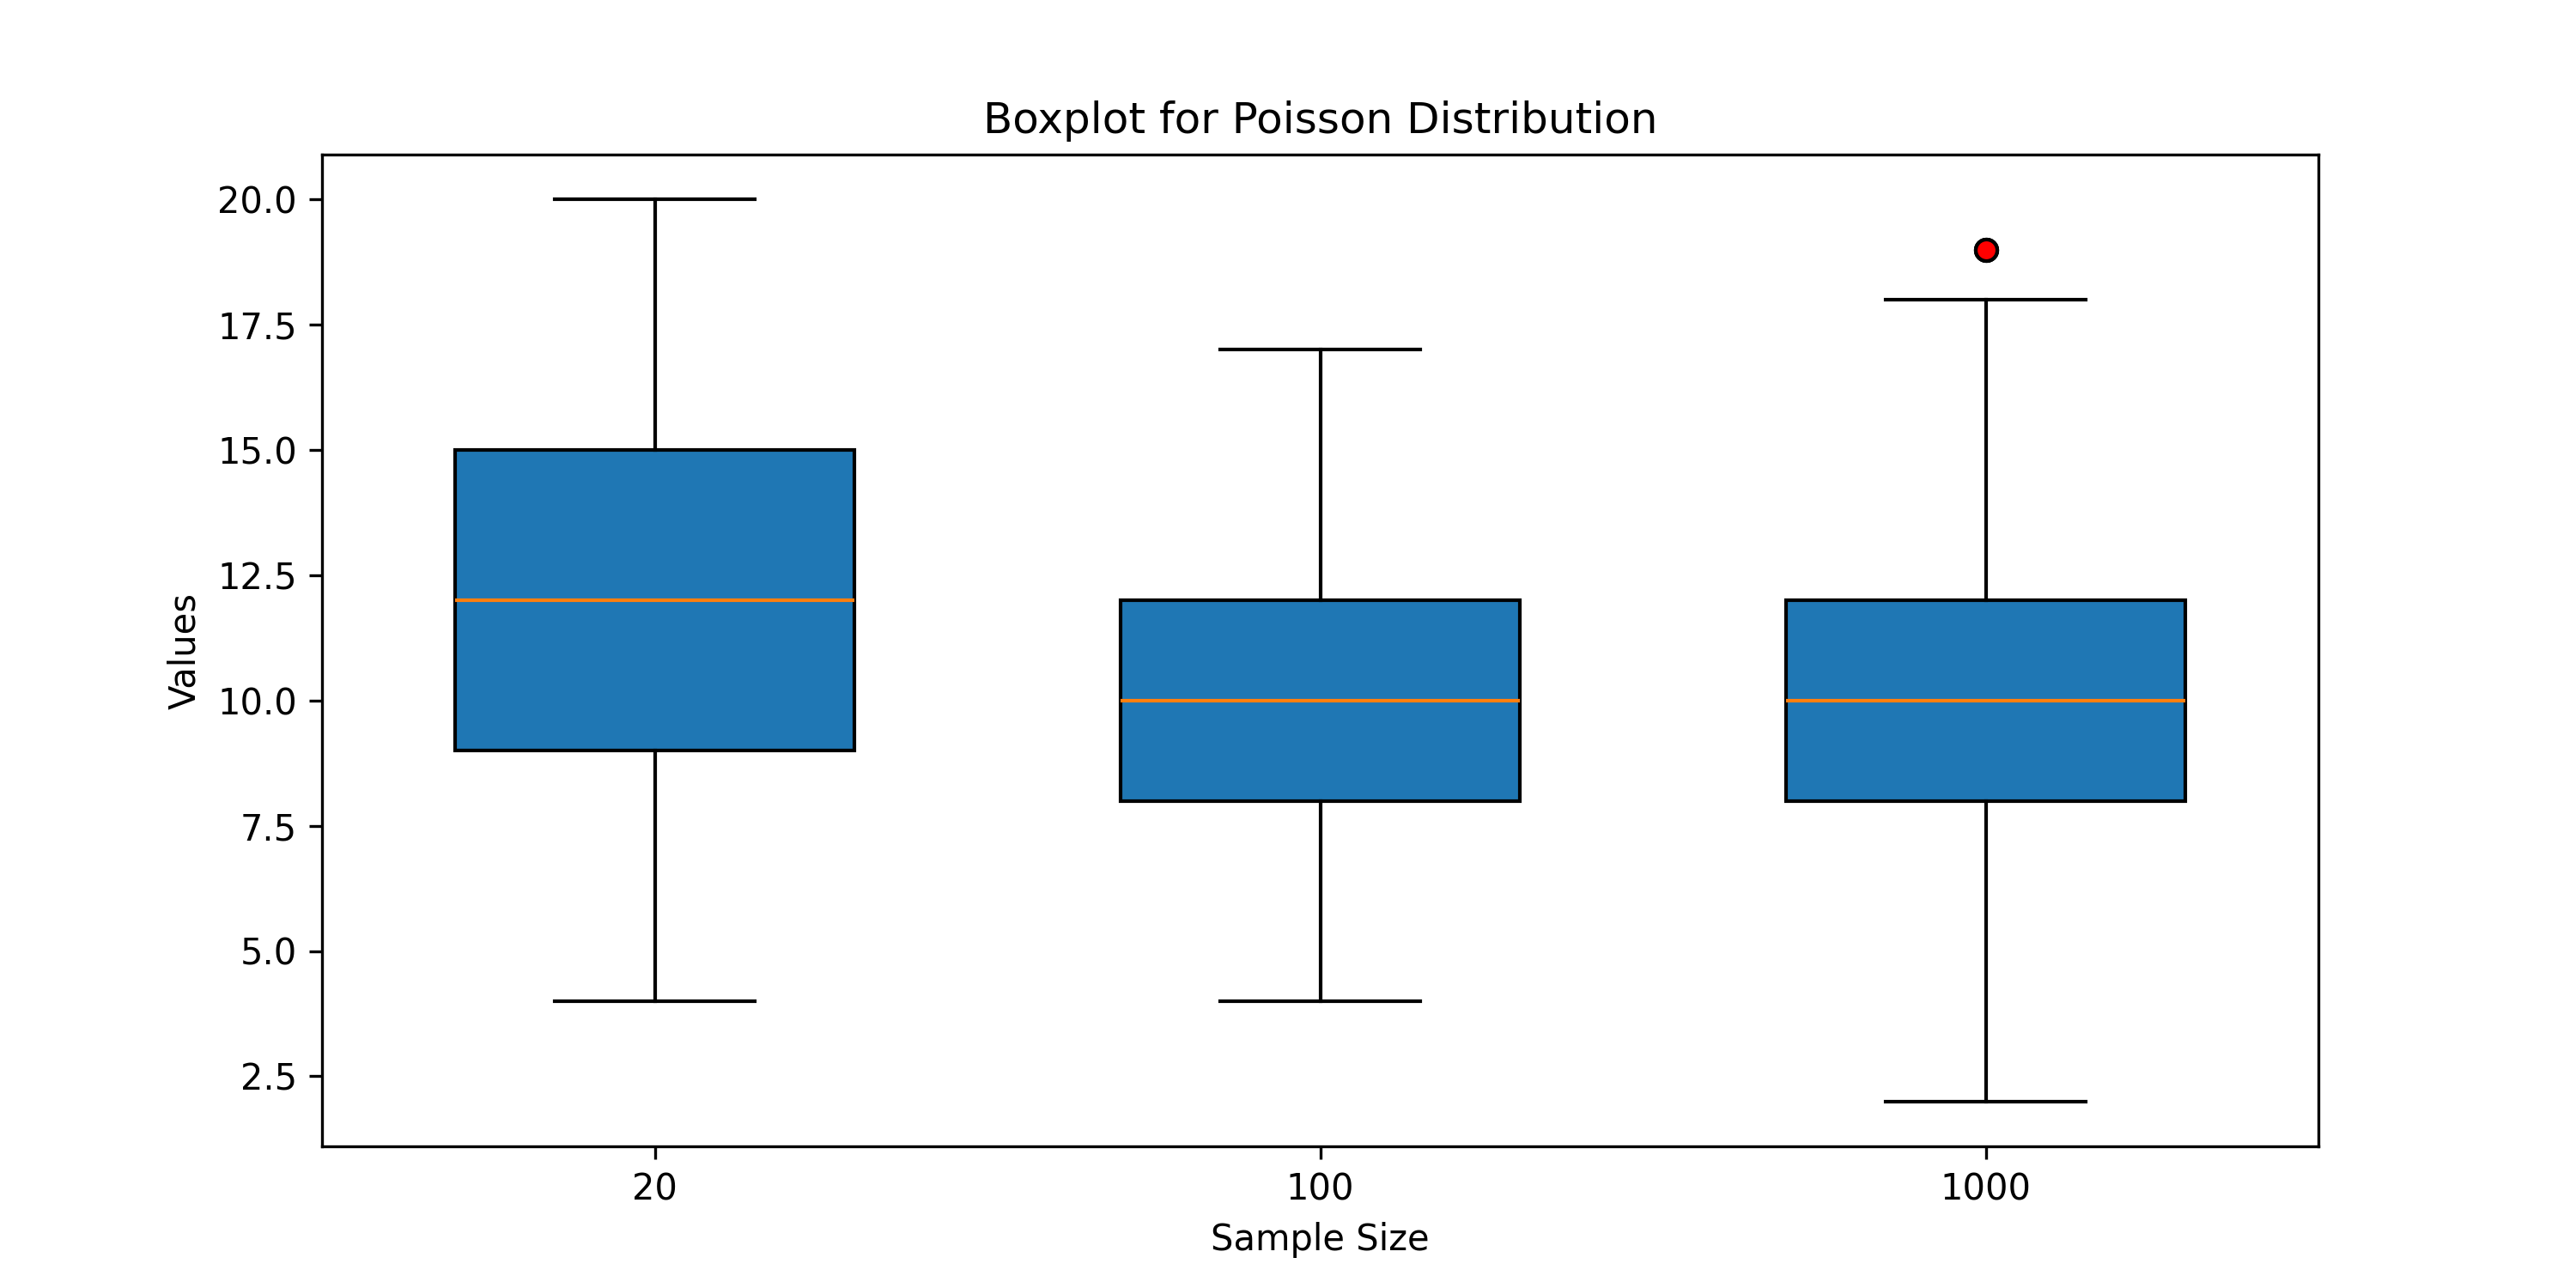
\includegraphics[width=0.8\textwidth]{./plots/poisson_boxplot}
        \caption{Боксплот Тьюки для распределения Пуассона}
        \label{fig:poisson_boxplot}
    \end{figure}

    \begin{figure}[H]
        \centering
        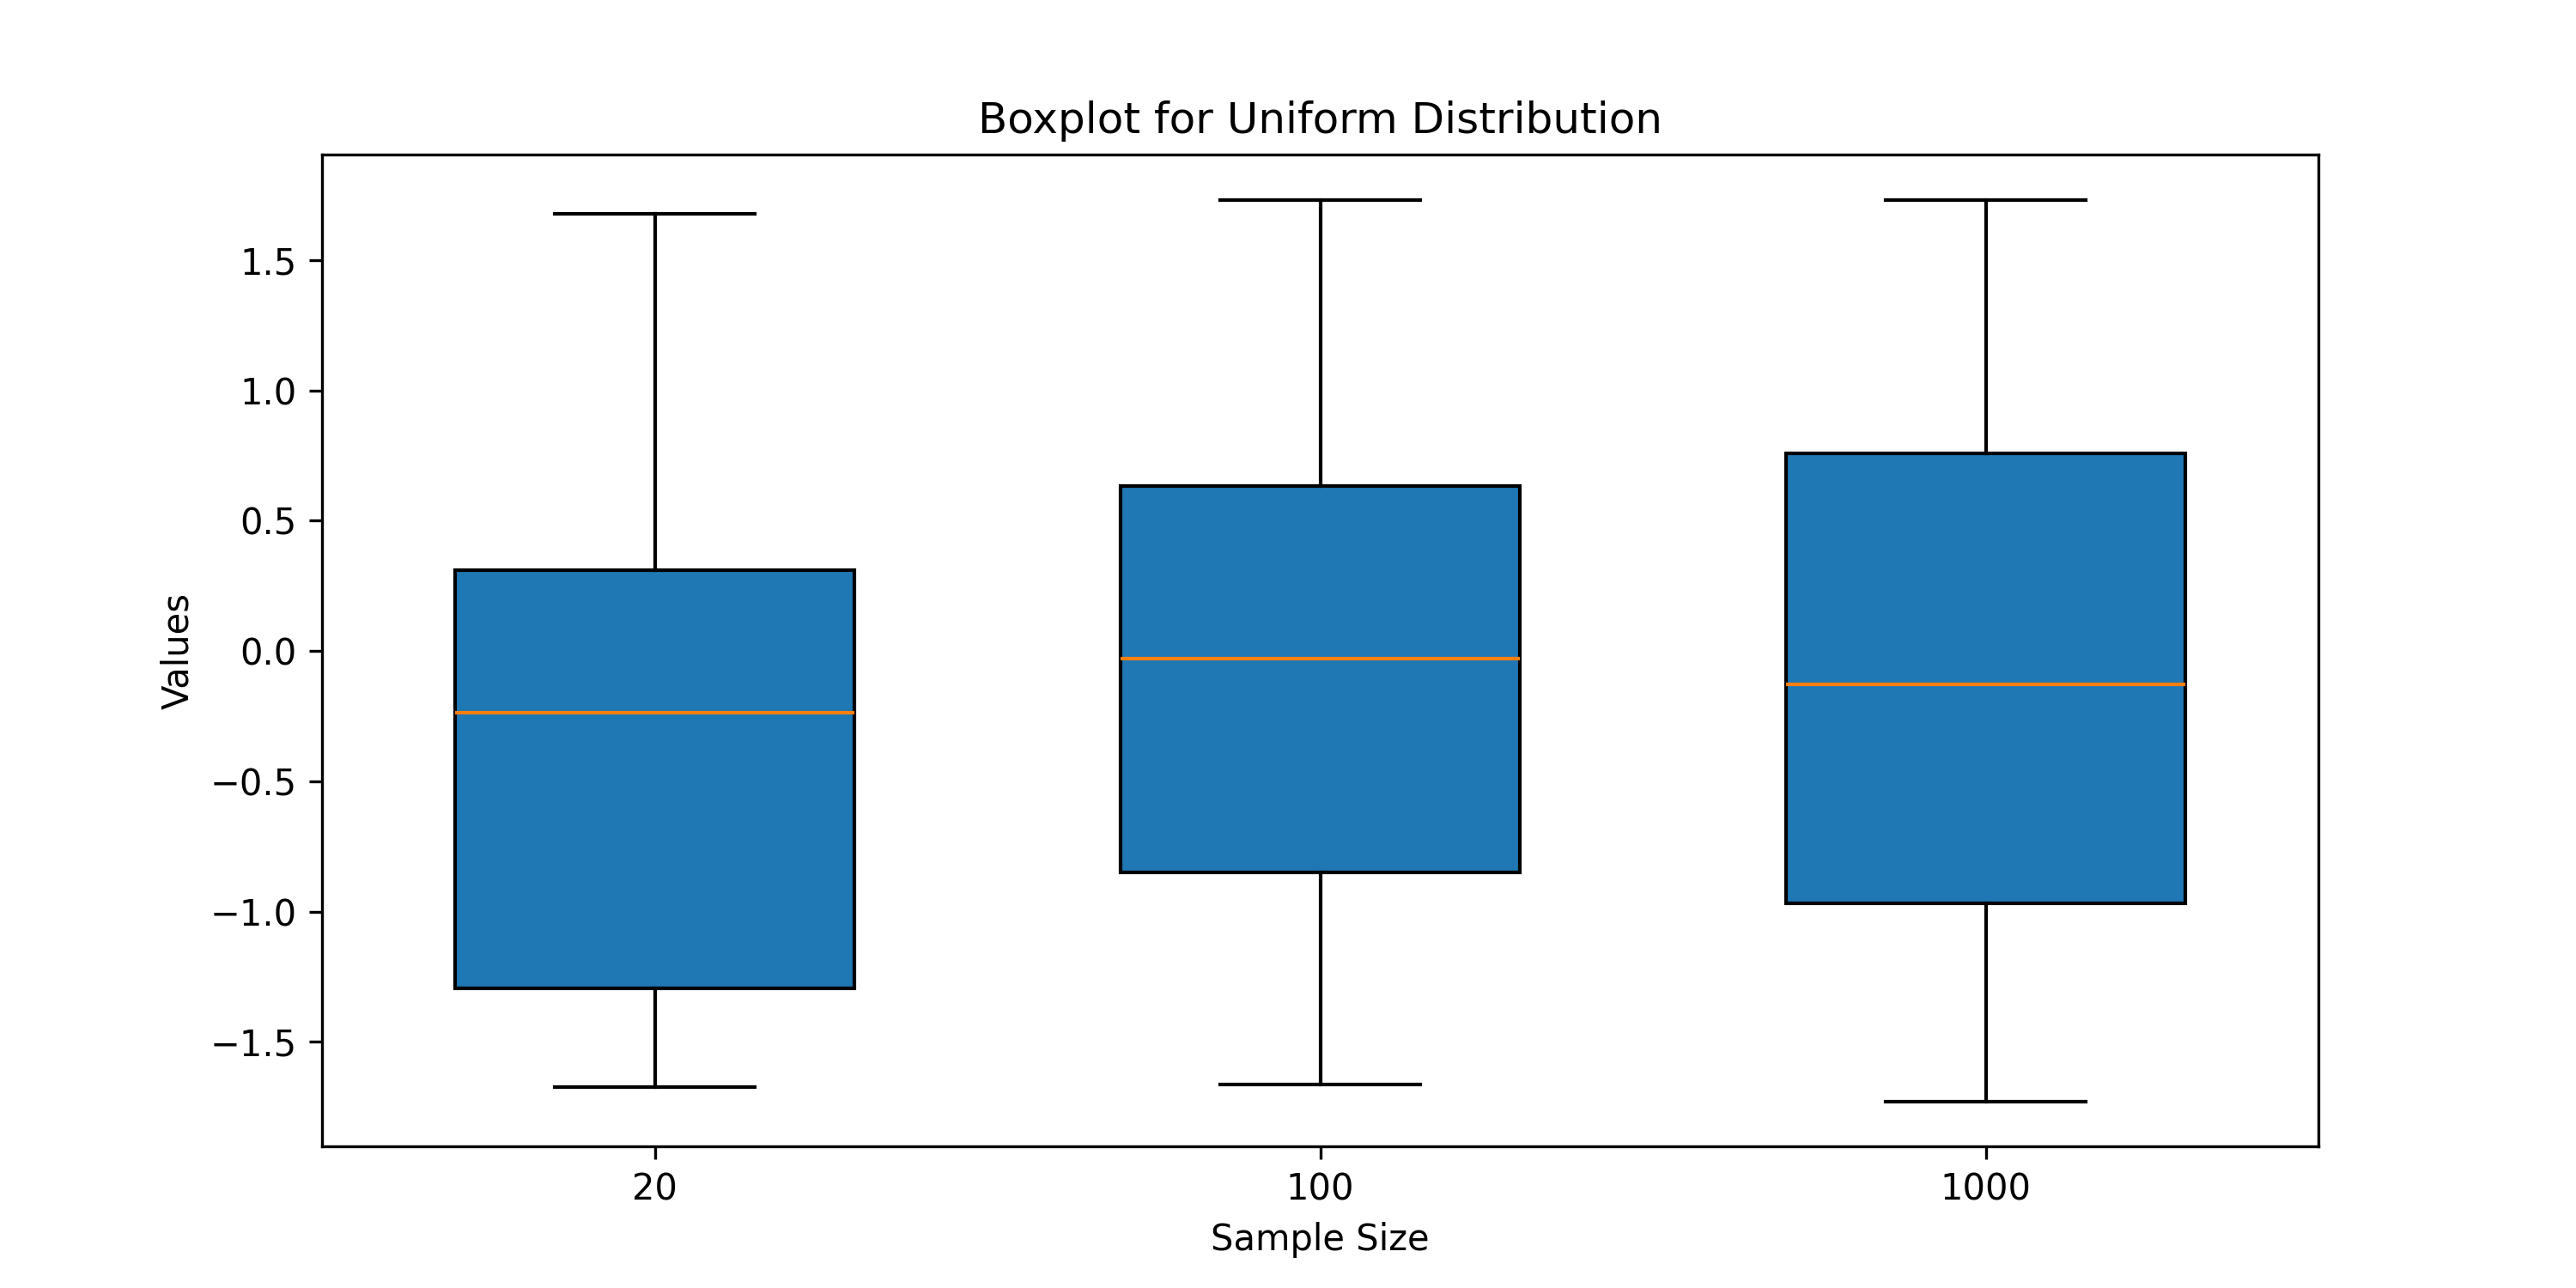
\includegraphics[width=0.8\textwidth]{./plots/uniform_boxplot}
        \caption{Боксплот Тьюки для равномерного распределения}
        \label{fig:uniform_boxplot}
    \end{figure}


    \section{Результаты анализа выбросов}\label{sec:outliers}
    \begin{table}[!htbp]
        \centering
        \caption{Количество выбросов в выборках различных распределений}
        \begin{tabular}{|c|c|c|c|}
            \hline
            \textbf{Распределение} & \textbf{n=20} & \textbf{n=100} & \textbf{n=1000} \\
            \hline
            Нормальное             & 2             & 1              & 6               \\
            \hline
            Коши                   & 4             & 10             & 160             \\
            \hline
            Пуассон                & 2             & 0              & 5               \\
            \hline
            Равномерное            & 0             & 0              & 0               \\
            \hline
        \end{tabular}
        \label{tab:outliers}
    \end{table}


    \section{Выводы}\label{sec:conclusions}
    \begin{itemize}
        \item Нормальное распределение имеет небольшое количество выбросов, что ожидаемо.
        \item Распределение Коши демонстрирует значительное количество выбросов из-за тяжелых хвостов.
        \item Пуассоновское распределение имеет мало выбросов, так как значения сосредоточены около 10.
        \item Равномерное распределение не имеет выбросов, так как его значения строго ограничены интервалом.
    \end{itemize}

\end{document}
